\documentclass[a4paper,11pt,dvipdfmx]{ujarticle}

\usepackage{graphicx}
\usepackage{url}

\input{layout}

\title{日本におけるデジタル化の状況}
\author{G684172026 トウフィ}

\begin{document}

\maketitle

\section{ブロードバンドの整備状況}

OECDによるブロードバンド回線の普及に関する調査\cite{oecd}によると，
図\ref{fig:broadband}に示すように，日本における100人あたりの
モバイルブロードバンドの加入者数は190.5で，第1位になっている。
2位はエストニアで，3位は米国と続く。

\begin{figure}[htbp]
\centering
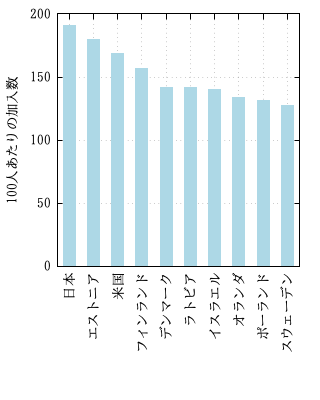
\includegraphics[width=0.5\linewidth]{fig21.png}
\caption{光ファイバー回線の加入者数（100人あたり）}
\label{fig:broadband}
\end{figure}

\section{デジタル競争力ランキング}

国際経営開発研究所（IMD）の調査\cite{imd}によると，
表\ref{tab:imd}に示すように，日本のデジタル競争力のランキングは
調査対象の64か国中，総合で28位，知識分野で25位となっている。

\begin{table}[htbp]
\centering
\caption{デジタル競争力ランキング（64カ国中）}
\label{tab:imd}

\begin{tabular}{|c|c|c|}
\hline
国 & 総合 & 知識 \\
\hline
米国 & 1位 & 3位 \\
\hline
香港 & 2位 & 5位 \\
\hline
スウェーデン & 3位 & 2位 \\
\hline
デンマーク & 4位 & 8位 \\
\hline
シンガポール & 5位 & 4位 \\
\hline
韓国 & 12位 & 15位 \\
\hline
中国 & 15位 & 6位 \\
\hline
日本 & 28位 & 25位 \\
\hline
\end{tabular}

\end{table}

\section{考察}

\begin{itemize}
\item 日本ではブロードバンドの普及率が高いことが分かった。
\item 一方で，デジタル競争力の総合順位は28位であり，通信環境の普及だけでは競争力の向上に十分ではないと考えられる。
\item 今後は，デジタル技術を活用できる人材の育成や，行政・企業での利用をさらに進める必要がある。
\end{itemize}

\bibliographystyle{junsrt}
\bibliography{exercise}

\end{document}